\documentclass[../main/Notes.tex]{subfiles}
\begin{document}

\section{Midterm Questions}\index{Midterm}
There are 8 questions and each question is worth 4 points. You only have to answer 6 out of the 8 questions. Hence, the maximum score is 24 points. If you answer more than 6 questions the answers with the lowest scores will be discarded. You have from 8:00 to 10:00 to work on your responses. Please respond in full sentences.

\subsection*{Question 1}\index{Bayes' Rule}
A. took an HIV test. The test turned out to be positive. About 0.01\% of men like him are infected with HIV. If someone has the virus there is a 99.9\% chance that the test result will be positive. If someone is not infected there is a 99.99\% chance that the result will be negative. What is the probability that A. is infected with HIV?

\subsection*{Question 2}
You have the choice of flying with a 2-engine or a 4-engine plane. Both are old models with the same kind of engines that sometimes fail with probability $p$. A plane can still fly if at least half of the engines are working. Which of the two is safer?

\subsection*{Question 3}
To encourage Elmer's promising tennis career, his father offers him a prize if he wins (at least) two tennis sets in a row in a three-set series to be played with his father and the club champion alternately: father-champion-father or champion-father-champion, according to Elmer's choice. The champion is a better player than Elmer's father. Which series should Elmer choose?

\subsection*{Question 4}\index{Odds}
Bookie A has set the odds for Real Madrid winning the Champions League to $1:3$ (i.e. if you bet 1\euro\ on Real Madrid you win 3\euro\ if Real Madrid wins) and the odds for Real Madrid not winning to $4:1$. Bookie B has set the odds for Madrid to $1:5$ and the odds against Madrid to $6:1$. How can you take advantage of this situation?

\subsection*{Question 5}
\begin{figure}[b]
  \centering
  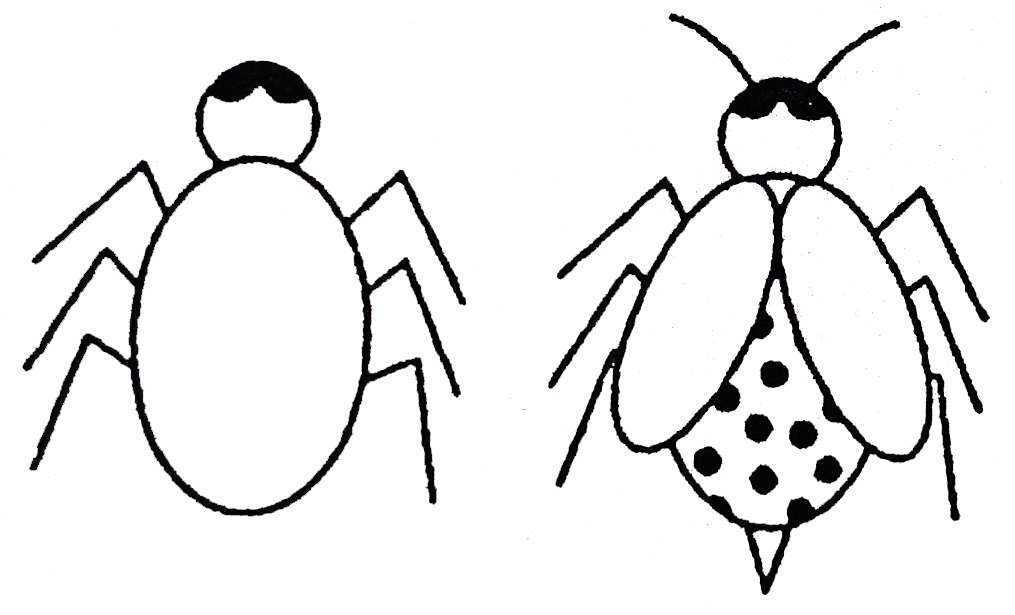
\includegraphics[width=2.5cm]{../images/bugs.jpg}
  \caption{Bugs}
  \label{fig:midterm_bugpic}
\end{figure}
In a simple word learning experiment subjects are shown bug-like stimuli. They can have wings or not, they can have antennas or not, they can have dots or not and they can have a sting or not (see figure \ref{fig:midterm_bugpic} for one bug that has none of these features and one bug that has all of these features). The experimenter picks one of the features uniformly at random, for example ``has wings''. The subject is told that they are learning a foreign language and that their task is to figure out what the word ``dax'' means. They are also told that the word ``dax'' refers to one of the four features (wings, antennas, dots, or sting) and that their task is to find out which one it is, for example ``has wings''. To this end, on every trial one of the 16 possible stimuli is picked by the experimenter uniformly at random and shown to the subject. The subject has to say whether the word ``dax'' applies to this stimulus or not. On each trial the experimenter gives feedback as to whether the word ``dax'' was used correctly or not, for example whether the stimulus has wings or not. Let's assume subjects have the following strategy: First, they pick one of the four features. They assume that this is the meaning of the word ``dax'' until they make a mistake. If they did not pick the right feature, how many trials will it take until they make a mistake (more precisely: What is the distribution over the number of trials that it takes)? If they made a mistake they will try the next feature. They don't try another feature unless they make a mistake. How many mistakes will they make until they found the correct interpretation of the word ``dax'' (i.e. what is the distribution over the number of mistakes)?

\subsection*{Question 6}\index{Change of variable}
$X$ is a continuous random variable with uniform probability density function
\begin{align*}
p(X=x)=\begin{cases}
e^{-x} &\text{for } 0 \leq x \\
0 & \text{otherwise}
\end{cases}
\end{align*}
What is the cumulative distribution function for $X$? $Y$ is a random variable that is defined as $Y=\sqrt{X}$. What is the cumulative distribution function of $Y$? What is the probability density function of $Y$?

\subsection*{Question 7}\index{Proper Scoring Rule}
Let $X$ be the truth-value of a statement (either 0 or 1). You want to elicit the beliefs of several experts about this statement. A friend of yours suggests to use the following loss function 
\begin{align*}
L(X,q) = -Xq^2-(1-X)(1-q)^2
\end{align*}
to score the responses (note that negative loss is gain). Is this loss function a proper scoring rule? Explain.

\subsection*{Question 8}\index{NHST}
The following are statements about p-values in published or online work. Explain why each is wrong and offer a correct version:
\begin{itemize}
	\item[(a)] ``If p < 0.05, the researcher knows that there is less than 1 chance in 20 that the observed difference between the experimental and control groups occurred by chance.''
  \item[(b)] ``A hypothesis is rejected if the probability that it is a true statement is very low - lower than some predetermined probability ... the level of significance.''
  \item[(c)] ``Significance levels show you how likely a result is due to chance. The most common level, used to mean something is good enough to be believed, is .95. This means that the finding has a 95\% chance of being true.''
  \item[(d)] ``By convention, a p-value higher than 0.05 usually indicates that the results of the study, however good or bad, were probably due only to chance.''
\end{itemize}

\end{document}